% main=pgfplots.tex

\section{User's Guide: Drawing Axes and Plots}
\subsection{\TeX-dialects: \LaTeX, Con{\TeX}t, plain \TeX }
\label{sec:tex:dialects}%
\PGFPlots\ is compatible with \LaTeX, Con{\TeX}t and plain \TeX. The only difference is how to specify environments. This affects any \PGF/\Tikz-environments and all \PGFPlots-environments like axis, semilogxaxis, semilogyaxis and loglogaxis:
\begin{description}
\def\HEAD{%
	\small
	%\lstset{boxpos=b,breaklines=false,aboveskip=3pt,belowskip=3pt}%
	%\hspace{-1cm}%
	\begin{tabular}{*{2}{p{4cm}}}%
}%
\item[\LaTeX:] |\usepackage{pgfplots}| and

{\HEAD
\begin{codeexample}[code only]
\begin{tikzpicture}
\begin{axis}
...
\end{axis}
\end{tikzpicture}
\end{codeexample}
&
\begin{codeexample}[code only]
\begin{tikzpicture}
\begin{semilogxaxis}
...
\end{semilogxaxis}
\end{tikzpicture}
\end{codeexample}
\\
\end{tabular}%
}

\begin{codeexample}[code only]
\documentclass[a4paper]{article}

% for dvipdfm:
%\def\pgfsysdriver{pgfsys-dvipdfm.def}
\usepackage{pgfplots}
\pgfplotsset{compat=1.3}% <-- moves axis labels near ticklabels (respects tick label widths)

\begin{document}
\begin{figure}
	\centering
	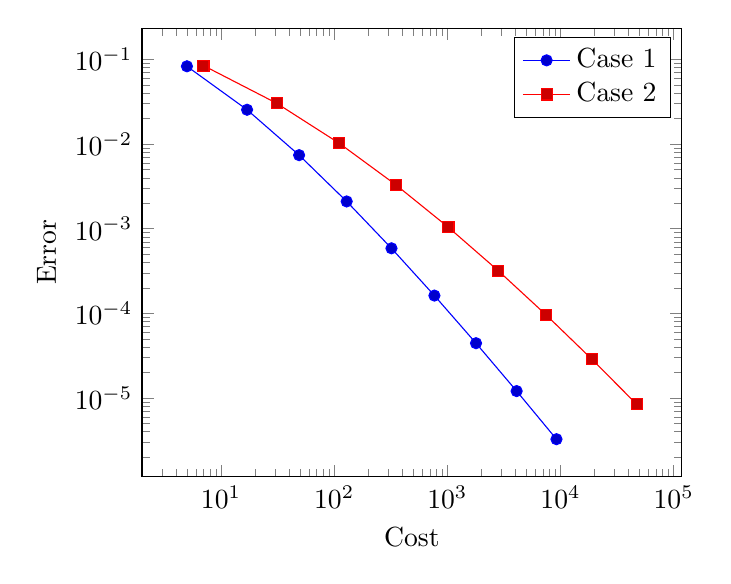
\begin{tikzpicture}
		\begin{loglogaxis}[xlabel=Cost,ylabel=Error]
		\addplot coordinates {
			(5,     8.31160034e-02)
			(17,    2.54685628e-02)
			(49,    7.40715288e-03)
			(129,   2.10192154e-03)
			(321,   5.87352989e-04)
			(769,   1.62269942e-04)
			(1793,  4.44248889e-05)
			(4097,  1.20714122e-05)
			(9217,  3.26101452e-06)
		};
		\addplot coordinates {
			(7,     8.47178381e-02)
			(31,    3.04409349e-02)
			(111,   1.02214539e-02)
			(351,   3.30346265e-03)
			(1023,  1.03886535e-03)
			(2815,  3.19646457e-04)
			(7423,  9.65789766e-05)
			(18943, 2.87339125e-05)
			(47103, 8.43749881e-06)
		};
		\legend{Case 1,Case 2}
		\end{loglogaxis}
	\end{tikzpicture}
	\caption{A larger example}
\end{figure}
\end{document}
\end{codeexample}

\item[Con{\TeX}t:] |\usemodule[pgfplots]| and

{\HEAD
\begin{codeexample}[code only]
\starttikzpicture
\startaxis
...
\stopaxis
\stoptikzpicture
\end{codeexample}
&
\begin{codeexample}[code only]
\starttikzpicture
\startsemilogxaxis
...
\stopsemilogxaxis
\stoptikzpicture
\end{codeexample}
\\
\end{tabular}%
}

A complete Con{\TeX}t--example file can be found in
\begin{codeexample}[code only]
doc/context/pgfplots/pgfplotsexample.tex.
\end{codeexample}

\item[plain \TeX:] |\input pgfplots.tex| and

{\HEAD
\begin{codeexample}[code only]
\tikzpicture
\axis
...
\endaxis
\endtikzpicture
\end{codeexample}
&
\begin{codeexample}[code only]
\tikzpicture
\semilogxaxis
...
\endsemilogxaxis
\endtikzpicture
\end{codeexample}
\\
\end{tabular}%
}

A complete plain--\TeX--example file can be found in
\begin{codeexample}[code only]
doc/plain/pgfplots/pgfplotsexample.tex.
\end{codeexample}
\end{description}
The default system drivers for |dvips| and |pdftex| work without any additional work; for |dvipdfm|, the |pgfsysdriver| macro needs to be redefined manually (see also section~\ref{sec:drivers}).


\subsection{A First Plot}
Plotting is done using \lstinline|\begin{axis} ... \addplot ...; \end{axis}|, where |\addplot| is the main interface to perform plotting operations.
\begin{codeexample}[]
\begin{tikzpicture}
	\begin{axis}[
		xlabel=Cost,
		ylabel=Error]
	\addplot[color=red,mark=x] coordinates {
		(2,-2.8559703)
		(3,-3.5301677)
		(4,-4.3050655)
		(5,-5.1413136)
		(6,-6.0322865)
		(7,-6.9675052)
		(8,-7.9377747)
	};
	\end{axis}
\end{tikzpicture}
\end{codeexample}


\begin{codeexample}[]
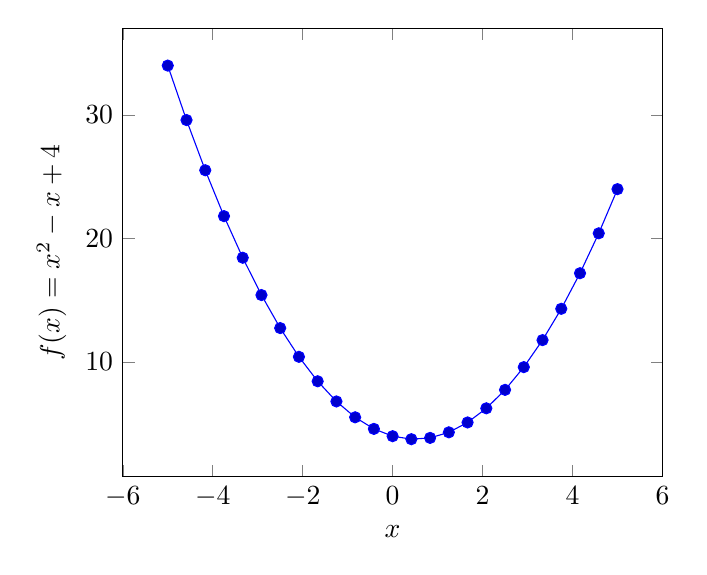
\begin{tikzpicture}
	\begin{axis}[
		xlabel=$x$,
		ylabel={$f(x) = x^2 - x +4$}
	]
	% use TeX as calculator:
	\addplot {x^2 - x +4};
	\end{axis}
\end{tikzpicture}
\end{codeexample}

\begin{codeexample}[]
\begin{tikzpicture}
	\begin{axis}[
		xlabel=$x$,
		ylabel=$\sin(x)$
	]
	% invoke external gnuplot as
	% calculator:
	\addplot gnuplot[id=sin]{sin(x)};
	\end{axis}
\end{tikzpicture}
\end{codeexample}

The |plot coordinates|, |plot expression| and |plot gnuplot| commands are three of the several supported ways to create plots, see section~\ref{sec:addplot} for more details\footnote{Please note that you need \lstinline{gnuplot} installed to use \lstinline{plot gnuplot}.} and the remaining ones (|plot file|, |plot shell|, |plot table| and |plot graphics|). The options `|xlabel|' and `|ylabel|' define axis descriptions.

\subsection{Two Plots in the Same Axis}
Multiple |\addplot|-commands can be placed into the same axis.
	% generated with this statement:
	%\addplot plot[id=filesuffix_noise,domain=-6:5,samples=10] gnuplot{(-x**5 - 242 + (-300 + 600*rand(0)))};
\begin{codeexample}[leave comments]
\begin{tikzpicture}
	\begin{axis}[
		height=9cm,
		width=9cm,
		grid=major,
	]
		
	\addplot gnuplot[id=filesuffix]{(-x**5 - 242)};
	\addlegendentry{model}

	\addplot coordinates {
		(-4.77778,2027.60977)
		(-3.55556,347.84069)
		(-2.33333,22.58953)
		(-1.11111,-493.50066)
		(0.11111,46.66082)
		(1.33333,-205.56286)
		(2.55556,-341.40638)
		(3.77778,-1169.24780)
		(5.00000,-3269.56775)
	};
	\addlegendentry{estimate}
	\end{axis}
\end{tikzpicture}
\end{codeexample}
A legend entry is generated if there are |\addlegendentry| commands (or one |\legend| command).

\subsection{Logarithmic Plots}
Logarithmic plots show $\log x$ versus $\log y$  (or just one logarithmic axis). \PGFPlots\ normally uses the natural logarithm, i.e. basis $e\approx2.718$ (see the key |log basis x|). Now, the axis description also contains minor ticks and the labels are placed at $10^i$.
\begin{codeexample}[]
\begin{tikzpicture}
\begin{loglogaxis}[xlabel=Cost,ylabel=Gain]
\addplot[color=red,mark=x] coordinates {
	(10,100)
	(20,150)
	(40,225)
	(80,340)
	(160,510)
	(320,765)
	(640,1150)
};
\end{loglogaxis}
\end{tikzpicture}
\end{codeexample}
A common application is to visualise scientific data. This is often provided in the format $1.42\cdot10^4$, usually written as 1.42e+04. Suppose we have a numeric table named |pgfplots.testtable|, containing
\begin{codeexample}[code only,tabsize=6]
Level Cost  Error
1     7     8.471e-02
2     31    3.044e-02
3     111   1.022e-02
4     351   3.303e-03
5     1023  1.038e-03
6     2815  3.196e-04
7     7423  9.657e-05
8     18943 2.873e-05
9     47103 8.437e-06
\end{codeexample}
then we can plot |Cost| versus |Error| using
\begin{codeexample}[]
\begin{tikzpicture}
\begin{loglogaxis}[
	xlabel=Cost,
	ylabel=Error]
\addplot[color=red,mark=x] coordinates {
	(5,    8.31160034e-02)
	(17,   2.54685628e-02)
	(49,   7.40715288e-03)
	(129,  2.10192154e-03)
	(321,  5.87352989e-04)
	(769,  1.62269942e-04)
	(1793, 4.44248889e-05)
	(4097, 1.20714122e-05)
	(9217, 3.26101452e-06)
};

\addplot[color=blue,mark=*] 
	table[x=Cost,y=Error] {pgfplots.testtable};

\legend{Case 1,Case 2}
\end{loglogaxis}
\end{tikzpicture}
\end{codeexample}
The first plot employs inline coordinates; the second one reads numerical data from file and plots column `|Cost|' versus `|Error|'.

\noindent
Besides the environment ``|loglogaxis|'' you can use
\begin{itemize}
	\item |\begin{axis}...\end{axis}| for normal plots,
	\item |\begin{semilogxaxis}...\end{semilogxaxis}| for plots which have a normal~$y$ axis and a logarithmic~$x$ axis,
	\item |\begin{semilogyaxis}...\end{semilogyaxis}| the same with $x$~and~$y$ switched,
	\item |\begin{loglogaxis}...\end{loglogaxis}| for double--logarithmic plots.
\end{itemize}
You can also use
\begin{codeexample}[code only]
\begin{axis}[xmode=normal,ymode=log]
...
\end{axis}
\end{codeexample}
which is the same as |\begin{semilogyaxis}...\end{semilogyaxis}|.
\begin{codeexample}[]
\begin{tikzpicture}
	\begin{semilogyaxis}[
		xlabel=Index,ylabel=Value]

	\addplot[color=blue,mark=*] coordinates {
		(1,8)
		(2,16)
		(3,32)
		(4,64)
		(5,128)
		(6,256)
		(7,512)
	};
	\end{semilogyaxis}%
\end{tikzpicture}%
\end{codeexample}

\subsection{Cycling Line Styles}
You can skip the style arguments for |\addplot[...]| to determine plot specifications from a predefined list:
\label{page:plotcoords:src}%
\pgfmanualpdflabel{\textbackslash plotcoords}{}%
\begin{codeexample}[width=4cm]
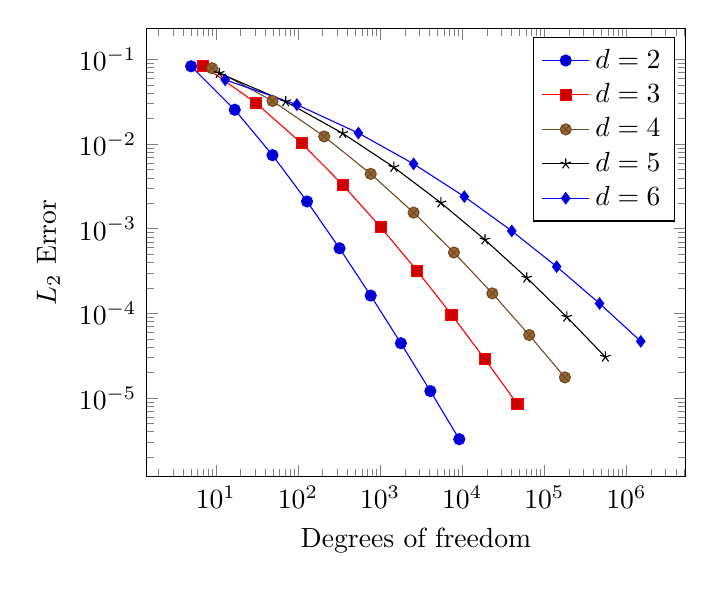
\begin{tikzpicture}
\begin{loglogaxis}[
	xlabel={Degrees of freedom},
	ylabel={$L_2$ Error}
]
\addplot coordinates {
	(5,8.312e-02)    (17,2.547e-02)   (49,7.407e-03)
	(129,2.102e-03)  (321,5.874e-04)  (769,1.623e-04)
	(1793,4.442e-05) (4097,1.207e-05) (9217,3.261e-06)
};

\addplot coordinates{
	(7,8.472e-02)    (31,3.044e-02)    (111,1.022e-02)
	(351,3.303e-03)  (1023,1.039e-03)  (2815,3.196e-04)
	(7423,9.658e-05) (18943,2.873e-05) (47103,8.437e-06)
};

\addplot coordinates{
	(9,7.881e-02)     (49,3.243e-02)    (209,1.232e-02)
	(769,4.454e-03)   (2561,1.551e-03)  (7937,5.236e-04)
	(23297,1.723e-04) (65537,5.545e-05) (178177,1.751e-05)
};

\addplot coordinates{
	(11,6.887e-02)    (71,3.177e-02)     (351,1.341e-02)
	(1471,5.334e-03)  (5503,2.027e-03)   (18943,7.415e-04)
	(61183,2.628e-04) (187903,9.063e-05) (553983,3.053e-05)
};

\addplot coordinates{
	(13,5.755e-02)     (97,2.925e-02)     (545,1.351e-02)
	(2561,5.842e-03)   (10625,2.397e-03)  (40193,9.414e-04)
	(141569,3.564e-04) (471041,1.308e-04) (1496065,4.670e-05)
};
\legend{$d=2$,$d=3$,$d=4$,$d=5$,$d=6$}
\end{loglogaxis}
\end{tikzpicture}
\end{codeexample}
\noindent
The |cycle list| can be modified, see the reference below.

\subsection{Scaling Plots}
You can use any of the \Tikz\ options to modify the appearance. For example, the ``|scale|'' transformation takes the picture as such and scales it.

\begin{codeexample}[]
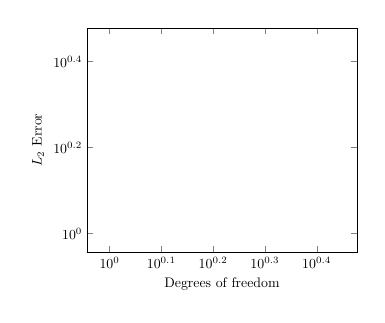
\begin{tikzpicture}[scale=0.5]
	\begin{loglogaxis}[
		xlabel={Degrees of freedom},
		ylabel={$L_2$ Error}
	]
	\plotcoords
	\legend{$d=2$,$d=3$,$d=4$,$d=5$,$d=6$}
	\end{loglogaxis}
\end{tikzpicture}

\begin{tikzpicture}[scale=1.1]
	\begin{loglogaxis}[
		xlabel={Degrees of freedom},
		ylabel={$L_2$ Error}
	]
	\plotcoords
	\legend{$d=2$,$d=3$,$d=4$,$d=5$,$d=6$}
	\end{loglogaxis}
\end{tikzpicture}
\end{codeexample}
However, you can also scale plots by assigning a |width=5cm| and/or |height=3cm| argument. This only affects the distance of point coordinates, no font sizes or axis descriptions:
\begin{codeexample}[]
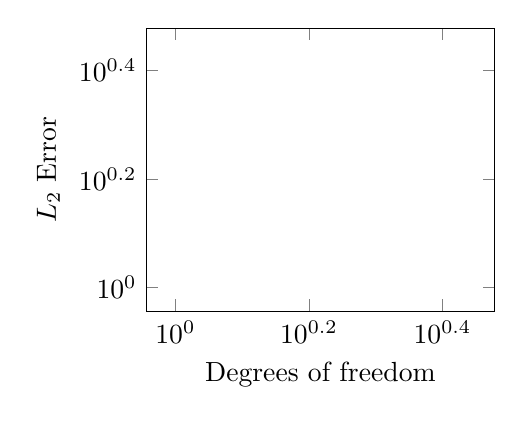
\begin{tikzpicture}
	\begin{loglogaxis}[
		width=6cm,
		xlabel={Degrees of freedom},
		ylabel={$L_2$ Error}
	]
	\plotcoords
	\legend{$d=2$,$d=3$,$d=4$,$d=5$,$d=6$}
	\end{loglogaxis}
\end{tikzpicture}

\begin{tikzpicture}
	\begin{loglogaxis}[
		width=8cm,
		xlabel={Degrees of freedom},
		ylabel={$L_2$ Error}
	]
	\plotcoords
	\legend{$d=2$,$d=3$,$d=4$,$d=5$,$d=6$}
	\end{loglogaxis}
\end{tikzpicture}
\end{codeexample}

Use the predefined styles |normalsize|, |small|, |footnotesize| to adopt font sizes and ticks automatically.

\endinput
